\documentclass[preview=false]{standalone}

\usepackage{color}
\usepackage{tikz}
\usepackage{pgfplots}
\definecolor{mcfblue}{rgb}{0,0.8,1}
\definecolor{mcforange}{rgb}{1,0.6,0}
\definecolor{mcfgreen}{rgb}{.68,.81,0}
\definecolor{mcfgrey}{gray}{0.95}
\definecolor{mcforange2}{rgb}{1,0.8,0}
\definecolor{mcforange3}{rgb}{1,0.2,0}

\begin{document}

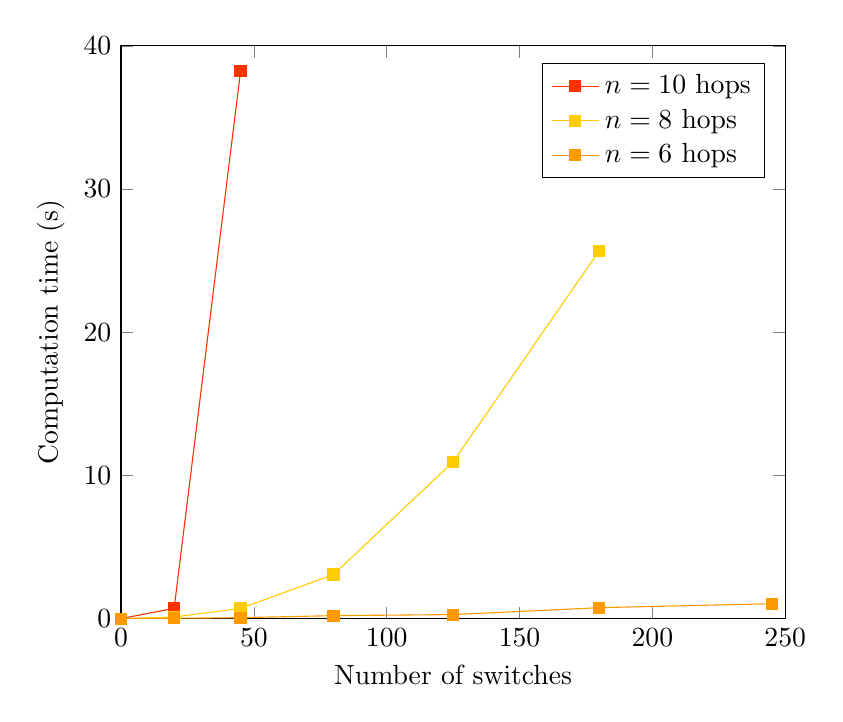
\begin{tikzpicture}
  \begin{axis}[
    xlabel = Number of switches,
    ylabel = Computation time (s),
    xmin=0, xmax=250, ymin=0, ymax=40,
    scale only axis,
    legend pos=north east,
    legend cell align=left
  ]

  \addplot[
    mark=square*, mcforange3, draw=mcforange3, 
    error bars/.cd, y dir=both, y explicit
  ]
  table[x=x,y=y,y error=yerr]
  {
    x       y        yerr
    0 0 0
    20  0.7256292 0.0070739045
    45  38.23024  0.1366292663
  };
  \addlegendentry{$n=10$ hops}

  \addplot[
    mark=square*, mcforange2, draw=mcforange2,
    error bars/.cd, y dir=both, y explicit
  ]
  table[x=x,y=y,y error=yerr]
  {
    x       y        yerr
    0 0 0 
    20  0.1143344 0.0027257511
    45  0.7122406 0.0030605062
    80  3.0836048 0.0217548799
    125 10.9429072  0.011007954
    180 25.692701 0.2385566181
  };
  \addlegendentry{$n=8$ hops}


  \addplot[
    mark=square*, mcforange, draw=mcforange,
    error bars/.cd, y dir=both, y explicit
  ]
  table[x=x,y=y,y error=yerr]
  {
    x       y        yerr
    0 0 0 
    20  0.0277476 0.0003812801
    45  0.06633 0.0036184659
    80  0.2110152 0.005928307
    125 0.283254  0.0053192575
    180 0.7664158 0.0074985986
    245 1.042033  0.0053563215
  };
  \addlegendentry{$n=6$ hops}

  \end{axis}
\end{tikzpicture}

\end{document}
